\section{赤道波动的数学框架}
\label{sec:framework}

本节将试图建立描述赤道波动的统一数学框架。
我们从三维层结大气的基本方程组出发，在赤道 $\beta$ 平面近似及其他合理近似下，将复杂的地球物理流体动力学问题转化为可解析求解的线性偏微分方程组。
其核心在于利用分离变量法，将三维问题分解为垂直方向的 Sturm-Liouville 本征值问题与水平方向的浅水波动方程，并通过算子代数方法揭示解空间的数学结构。
这一框架为第 \ref{sec:waves} 节的模态分析和第 \ref{sec:perturbation} 节的微扰论处理提供了必要的数学基础。

\subsection{基本方程组}
\label{subsec:primitive_equations}

考虑在旋转球面上运动的层结流体，采用局地笛卡尔坐标系 $(x, y, z)$，其中 $x$ 为纬向（向东为正），$y$ 为经向（向北为正），$z$ 为垂向。
层结大气的基本方程组包括动量方程、连续性方程和热力学方程。
为便于求解，以下采取一些假设来简化推导，并滤去一些难以解析计算的波。

我们所关注的大尺度赤道波动，其水平特征尺度（$10^3$ km 量级）远大于垂直特征尺度（$10$ km 量级）。
尺度分析表明，垂直方向的加速度量级远小于重力加速度与垂直气压梯度力，因此可以忽略垂直动量方程中的加速度项，认为垂直气压梯度力与重力始终保持平衡，即静力平衡。
该近似有效地滤除了高频波，保留了对天气和气候具有重要意义的低频波动模态，垂直动量方程简化为：
\begin{equation}
    \pde{\pressure}{z} = -\density \gravityconst
    \label{eq:hydrostatic}
\end{equation}

针对赤道区域，科氏参数 $\coriolis$ 可在赤道 $\latitude = 0$ 处进行泰勒展开。
忽略高阶项，仅保留线性项 $\coriolis \approx \beta y$，其中 $\rossby$ 为 Rossby 参数。
即得到赤道 $\beta$ 平面近似：
\begin{equation}
    \coriolis = 2\norm{\rotationvec} \sin\latitude \approx \rossby y, \quad \rossby = \frac{2\norm{\rotationvec}}{\earthradius}
    \label{eq:beta_plane}
\end{equation}

该近似简化了科氏力的数学形式。
科氏力随纬度线性增加的恢复机制，是构成赤道波导的动力学基础。
正如 \citep{matsunoQuasiGeostrophicMotionsEquatorial1966} 所指出的，这种线性变化的科氏参数使得波动能量被有效地束缚在赤道附近的狭窄纬带内，形成一种类似于量子力学中势阱约束的几何结构。
波动能量被束缚在了赤道附近的波导区内，这正是赤道波动得以长距离维持的关键机制。

假设大气处于静止基态（$\vel_0 = \ivec{0}$），且满足水平均匀条件，即背景密度 $\density_0(z)$、背景压强 $\pressure_0(z)$ 与背景位温 $\ptemp_0(z)$ 仅随高度变化。
为便于解析求解，通常假设背景密度随高度呈指数衰减：
\begin{equation}
    \density_0(z) = \density_s \ee^{-z/\scaleheight}
    \label{eq:background_density}
\end{equation}

其中 $\density_s$ 为地表参考密度，$\scaleheight$ 为大气标高。
这一假设确立了波动的传播介质环境，使得我们可以专注于波动本身的演变而无需顾虑背景流场的复杂性。

在自由大气中，大尺度波动的演变主要受惯性力、压力梯度力与科氏力的支配。
因此，我们忽略分子粘性及湍流摩擦耗散项。

将瞬时物理量分解为基态与小扰动量之和，并忽略扰动量的二阶及高阶项，则在无粘条件下，线性化的基本方程组可写为：

\textbf{水平动量方程}
\begin{align}
    \pde{u}{\timevar} - \rossby y v &= -\frac{1}{\density_0}\pde{\pressure}{x} \label{eq:momentum_u} \\
    \pde{v}{\timevar} + \rossby y u &= -\frac{1}{\density_0}\pde{\pressure}{y} \label{eq:momentum_v}
\end{align}

\textbf{连续性方程}
\begin{equation}
    \pde{u}{x} + \pde{v}{y} + \frac{1}{\density_0}\pde{(\density_0 w)}{z} = 0
    \label{eq:continuity}
\end{equation}

\textbf{热力学方程}
\begin{equation}
    \pde{\ptemp^\prime}{\timevar} + w \ode{\ptemp_0}{z} = \frac{\ptemp_0}{\gravityconst} \nonadheat
    \label{eq:thermodynamic}
\end{equation}

上述各式中扰动量的上标已省略以简化记号。
其中热力学方程 \eqref{eq:thermodynamic} 中的 $\nonadheat$ 是归一化的非绝热加热率。
线性化处理使得方程组适用叠加原理，复杂的实际大气扰动可以视为不同线性本征模态的叠加。

\subsection{非绝热加热的物理意义}
\label{subsec:heating_interpretation}

热力学方程 \eqref{eq:thermodynamic} 中的 $\nonadheat$ 是连接干大气动力学与湿对流过程的关键纽带。
理解此项的物理意义，对于后续章节中干波与湿波的讨论至关重要。

在理想的干大气模型中，$\nonadheat = 0$，波动由纯粹的动力学机制所驱动。
这一假设对于描述平流层中的波动现象是合理的，因为那里的水汽含量极低，潜热释放可以忽略不计。
早期的观测研究，如 \citep{Yanai1966} 和 \citep{Wallace1968} 在平流层中发现的混合 Rossby-重力波与 Kelvin 波，其传播特性均与干大气理论预测高度吻合。

然而，热带对流层中的情况则截然不同。
水汽相变释放的潜热是驱动大尺度环流的主要能量来源，因此必须考虑 $\nonadheat$ 的贡献。对于对流耦合赤道波（CCEWs），非绝热加热通常被参数化为波动自身动力场的函数。
一种广泛采用的方案是 Wave-CISK 参数化 \citep{lindzenWaveCISKTropics1974}，其基本假设是非绝热加热与低层水汽辐合（或等价地，与垂直上升运动）成正比。
在这种视角下，加热项不再是纯粹的外强迫，而是成为系统内部反馈机制的一部分。
数学形式为：
\begin{equation}
    \nonadheat = -\moistparam \bvfreq^2 w
    \label{eq:heating_param}
\end{equation}

其中 $\bvfreq \equiv (\gravityconst/\ptemp_0)(\mathrm{d}\ptemp_0/\mathrm{d}z)$ 是Brunt-Vaisala 频率，表征大气的静力稳定度。
$\moistparam \in [0, 1)$ 是表征耦合强度的无量纲参数。
当 $\moistparam = 0$ 时，系统退化为干大气极限；当 $\moistparam$ 接近 $1$ 时，加热与动力学之间的正反馈导致大气有效静力稳定度趋于零。
参数 $\moistparam$ 本质上是“总湿稳定度”（Gross Moist Stability, GMS）的归一化度量，它刻画了潜热释放对绝热冷却的抵消程度 \citep{kiladisConvectivelyCoupledEquatorial2009}。
关于加热参数化对波动性质的具体影响，我们将在第 \ref{sec:waves} 节中详细讨论。

\subsection{垂直与水平结构的分离}
\label{subsec:separation}

为求解上述方程组，引入扰动位势 $\gravpotential = \pressure^\prime / \density_0$。
利用线性化的静力平衡关系 $\partial \pressure^\prime/\partial z = -\density^\prime \gravityconst$ 以及状态方程 $\density^\prime/\density_0 \approx -\ptemp^\prime/\ptemp_0$，可以建立动力学变量 $\gravpotential$ 与热力学变量 $\ptemp^\prime$ 之间的诊断关系：
\begin{equation}
    \pde{\gravpotential}{z} \approx \frac{\gravityconst}{\ptemp_0} \ptemp^\prime
    \label{eq:hydrostatic_relation}
\end{equation}

这一关系表明，在静力平衡的大气中，局地的位温异常直接决定了等压面的厚度变化。
将上式代入热力学方程 \eqref{eq:thermodynamic}，并利用 Brunt-Vaisala 频率的定义，可消去 $\ptemp^\prime$，得到：
\begin{equation}
    \pde{}{\timevar}\left(\pde{\gravpotential}{z}\right) + \bvfreq^2 w = \nonadheat
    \label{eq:thermo_phi}
\end{equation}

我们首先讨论干大气条件下（$\nonadheat = 0$）的情形。
设物理量具有分离变量形式：
\begin{equation}
    \begin{pmatrix} u \\ v \\ \gravpotential \end{pmatrix}(x, y, z, \timevar)
    = \sum_{\vertmode=0}^{\infty}
    \begin{pmatrix} u_\vertmode \\ v_\vertmode \\ \gravpotential_\vertmode \end{pmatrix}(x, y, \timevar)
    \cdot \vertfunc_\vertmode(z)
    \label{eq:separation_ansatz}
\end{equation}

由 \eqref{eq:thermo_phi}，在干大气条件下垂直速度可表示为：
\begin{equation}
    w = -\frac{1}{\bvfreq^2}\pde{}{\timevar}\left(\pde{\gravpotential}{z}\right)
    \label{eq:w_from_phi}
\end{equation}

将此式代入连续性方程 \eqref{eq:continuity}，消去 $w$ 后得到：
\begin{equation}
    \pde{u}{x} + \pde{v}{y} - \frac{1}{\density_0}\pde{}{z}\left[\frac{\density_0}{\bvfreq^2}\pde{}{\timevar}\left(\pde{\gravpotential}{z}\right)\right] = 0
    \label{eq:combined_continuity}
\end{equation}

上式表明，垂直结构函数 $\vertfunc_\vertmode(z)$ 必须是特定算子的本征函数，才能使方程组具有分离变量解。
定义垂直结构算子 $\vertop$ 为：
\begin{equation}
    \vertop \equiv \frac{1}{\density_0(z)}\pde{}{z}\left(\frac{\density_0(z)}{\bvfreq^2(z)}\pde{}{z}\right)
    \label{eq:vertical_operator}
\end{equation}

则垂直方向的本征方程为：
\begin{equation}
    \vertop \vertfunc_\vertmode(z) = -\frac{1}{\gravityconst \eqdepth_\vertmode} \vertfunc_\vertmode(z)
    \label{eq:vertical_eigen}
\end{equation}

这里出现的本征值 $\eqdepth_\vertmode$ 即为等效深度（equivalent depth）。
该量具有长度量纲，是连接三维层结大气垂直结构与二维浅水模型水平波动的核心参数。
每一个特定的垂直模态 $\vertfunc_\vertmode(z)$ 对应一个确定的等效深度 $\eqdepth_\vertmode$，而等效深度又决定了该垂直模态在水平方向上的传播特性。

算子 $\vertop$ 在适当边界条件下的性质可由 Sturm-Liouville 理论加以刻画，参考 \citep{Magnus2023}。
在刚性边界条件（即地面与层顶处垂直速度为零，等价于 $\partial\vertfunc_\vertmode/\partial z = 0$）下，$\vertop$ 是自伴算子。
定义加权内积：
\begin{equation}
    \langle f, g \rangle \equiv \int_0^{z_T} f(z)\, g(z)\, \density_0(z)\, \mathrm{d}z
    \label{eq:inner_product}
\end{equation}

则算子的自伴性 $\langle f, \vertop g \rangle = \langle \vertop f, g \rangle$ 可通过分部积分验证。
由此，Sturm-Liouville 理论保证其本征值 $\{\eqdepth_\vertmode\}$ 均为正实数且构成离散谱，对应的本征函数族 $\{\vertfunc_\vertmode(z)\}$ 在加权内积下构成完备正交归一基。
这一性质保证了任意满足边界条件的垂直廓线都可以唯一地展开为本征函数的线性叠加。关于 Sturm-Liouville 理论的严格数学表述，请参阅附录 \ref{app:sturm_liouville}。

利用垂直本征函数的正交性，可将原始方程组投影到各个垂直模态上，从而得到一系列相互独立的水平结构方程组。
对于第 $\vertmode$ 个垂直模态（以下省略下标），其水平运动满足经典的浅水波动方程：
\begin{align}
    \pde{u}{\timevar} - \rossby y\, v &= -\pde{\gravpotential}{x} \label{eq:swe_u}\\
    \pde{v}{\timevar} + \rossby y\, u &= -\pde{\gravpotential}{y} \label{eq:swe_v}\\
    \pde{\gravpotential}{\timevar} + \ceq^2\left(\pde{u}{x} + \pde{v}{y}\right) &= 0 \label{eq:swe_phi}
\end{align}

其中 $\ceq = \sqrt{\gravityconst \eqdepth}$ 为重力波速度。
上述方程组形式上与单层流体的浅水方程完全一致，只是其中的自由表面高度被等效深度 $\eqdepth$ 所取代。
这一结果揭示了一个重要的物理图像：三维层结大气中的波动可以分解为一系列独立的二维浅水波的叠加，每一个浅水波对应于一个特定的垂直结构模态。
不同垂直模态之间的相互独立性源于本征函数的正交性，而它们在数学处理上的统一性则源于方程组形式的普适性。

\subsection{无量纲化与算子代数表示}
\label{subsec:operator_algebra}

为进一步分析水平结构方程组的解，引入无量纲化并采用算子代数方法。
这种处理方式类似于量子力学中谐振子问题的代数化求解，能够清晰地揭示解空间的数学结构。

基于等效深度 $\eqdepth$ 和 Rossby 参数 $\rossby$ 构造特征尺度：
\begin{equation}
    \Leq = \sqrt{\frac{\ceq}{\rossby}}, \quad \Teq = \frac{1}{\sqrt{\ceq\rossby}}, \quad \ceq = \sqrt{\gravityconst\eqdepth}
    \label{eq:natural_scales}
\end{equation}

其中 $\Leq$ 称为赤道变形半径（equatorial radius of deformation），刻画了波动在经向上的特征束缚宽度；$\Teq$ 则是相应的惯性时间尺度。
引入无量纲变量：
\begin{equation}
    x = \Leq\ndim{x}, \quad y = \Leq\ndim{y}, \quad \timevar = \Teq\ndim{\timevar}, \quad u = \ceq\ndim{u}, \quad v = \ceq\ndim{v}, \quad \gravpotential = \ceq^2\ndim{\gravpotential}
\end{equation}

代入方程 \eqref{eq:swe_u}--\eqref{eq:swe_phi}，省略波浪号，得到无量纲化的基本方程组：
\begin{align}
    \pde{u}{\timevar} - y\, v &= -\pde{\gravpotential}{x} \label{eq:nondim_u}\\
    \pde{v}{\timevar} + y\, u &= -\pde{\gravpotential}{y} \label{eq:nondim_v}\\
    \pde{\gravpotential}{\timevar} + \pde{u}{x} + \pde{v}{y} &= 0 \label{eq:nondim_phi}
\end{align}

进一步假设解具有纬向行波和简谐振荡的形式：
\begin{equation}
    (u, v, \gravpotential) = (\complexamp{u}(y), \complexamp{v}(y), \complexamp{\gravpotential}(y))\, \complexexp{\wavenum x - \frequency\timevar}
    \label{eq:wave_ansatz}
\end{equation}

其中 $\wavenum$ 为纬向波数，$\frequency$ 为角频率。
代入无量纲方程组后，得到关于经向振幅的代数系统：
\begin{align}
    -\ii\frequency\complexamp{u} - y\complexamp{v} &= -\ii\wavenum\complexamp{\gravpotential} \label{eq:spectral_u}\\
    -\ii\frequency\complexamp{v} + y\complexamp{u} &= -\ode{\complexamp{\gravpotential}}{y} \label{eq:spectral_v}\\
    -\ii\frequency\complexamp{\gravpotential} + \ii\wavenum\complexamp{u} + \ode{\complexamp{v}}{y} &= 0 \label{eq:spectral_phi}
\end{align}

引入梯算子（ladder operators）：
\begin{equation}
    \aop \equiv \frac{1}{\sqrt{2}}\left(\ode{}{y} + y\right), \quad \adop \equiv \frac{1}{\sqrt{2}}\left(-\ode{}{y} + y\right)
    \label{eq:ladder_operators}
\end{equation}

这两个算子满足对易关系 $\comm{\aop}{\adop} = 1$，与量子力学中的产生-湮灭算子代数同构。
定义数算子 $\Nop \equiv \adop\aop$，则谐振子哈密顿量可写为：
\begin{equation}
    \Hop \equiv \Nop + \frac{1}{2} = -\frac{1}{2}\ode[2]{}{y} + \frac{1}{2}y^2
    \label{eq:hamiltonian}
\end{equation}

通过定义组合变量：
\begin{equation}
    \qvar \equiv \frac{\complexamp{\gravpotential} + \complexamp{u}}{\sqrt{2}}, \quad \rvar \equiv \frac{\complexamp{\gravpotential} - \complexamp{u}}{\sqrt{2}}
    \label{eq:qr_def}
\end{equation}

方程组 \eqref{eq:spectral_u}--\eqref{eq:spectral_phi} 可重写为算子形式：
\begin{align}
    (\frequency - \wavenum)\qvar &= -\ii\adop\complexamp{v} \label{eq:q_eq}\\
    (\frequency + \wavenum)\rvar &= \ii\aop\complexamp{v} \label{eq:r_eq}\\
    \frequency\complexamp{v} &= \ii(\aop\qvar - \adop\rvar) \label{eq:v_eq}
\end{align}

该方程组非平凡解存在的条件即为频散关系，其求解可归结为数算子 $\Nop$ 的本征值问题。
$\Nop$ 的本征值为非负整数 $\modenum = 0, 1, 2, \ldots$，对应的本征函数是厄米函数（Hermite functions）：
\begin{equation}
    \hfunc{\modenum}(y) = \frac{1}{\sqrt{\sqrt{\pi}2^\modenum \modenum!}}\Hpoly{\modenum}(y)\,\ee^{-y^2/2}
    \label{eq:hermite_functions}
\end{equation}

\begin{figure}[htbp]
  \centering
  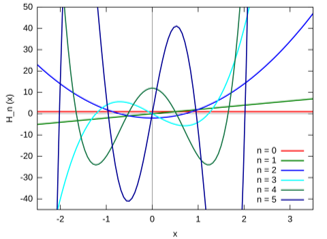
\includegraphics[width=0.8\linewidth]{assets/hermite.png}
  \caption{厄米函数在不同n取值下的图像。}
  \label{fig:Hermite}
\end{figure}

其中 $\Hpoly{\modenum}(y)$ 为 $\modenum$ 阶厄米多项式。
梯算子作用于厄米函数的规则为：
\begin{equation}
    \aop\hfunc{\modenum} = \sqrt{\modenum}\hfunc{\modenum-1}, \quad \adop\hfunc{\modenum} = \sqrt{\modenum+1}\hfunc{\modenum+1}
    \label{eq:ladder_action}
\end{equation}
其中约定 $\hfunc{-1} \equiv 0$。厄米函数族 $\{\hfunc{\modenum}(y)\}_{\modenum=0}^{\infty}$ 构成 $L^2(\mathbb{R})$ 空间的完备正交归一基，波动的经向结构可以唯一地展开为这些基函数的线性组合。

理解其物理意义，科氏参数的纬度变化 $\coriolis = \rossby y$ 在动力学上等效于二次型势阱 $V(y) = y^2/2$。
赤道是势阱中心，波动能量被束缚在了赤道附近，经向分布由厄米函数描述。

\subsection{解空间的结构}
\label{subsec:solution_space}

综合上述分析，赤道波动方程组的完整解空间 $\mathcal{H}$ 具有张量积结构：
\begin{equation}
    \mathcal{H} = \mathcal{H}_z \otimes \mathcal{H}_{xy}
    \label{eq:solution_space}
\end{equation}

其中 $\mathcal{H}_z = \mathrm{span}\{\vertfunc_\vertmode(z)\}_{\vertmode=0}^\infty$ 由垂直本征函数张成，$\mathcal{H}_{xy} = \mathrm{span}\{\hfunc{\modenum}(y)\ee^{\ii\wavenum x}\}_{\modenum=0}^\infty$ 由水平本征函数张成。

该解空间中的任一态可由三个量子数唯一标识。
第一个是垂直量子数 $\vertmode$，它决定了等效深度 $\eqdepth_\vertmode$ 的数值以及波动在垂直方向上的节点结构；较大的 $\vertmode$ 对应较小的等效深度和更复杂的垂直廓线。
第二个是经向量子数 $\modenum$，它决定了经向速度场的节点数目以及波动在赤道附近的空间形态；不同的 $\modenum$ 值还对应于不同类型的波动模态，如 Kelvin 波（形式上对应 $\modenum = -1$）、混合 Rossby-重力波（$\modenum = 0$）以及更高阶的 Rossby 波与惯性重力波。
第三个是纬向波数 $\wavenum$，它是连续参数，决定了波动在纬向上的传播方向与空间周期。
我们将在第 \ref{sec:waves} 节中详细讨论不同量子数组合对应的具体波动模态及其物理特性。

对于给定的 $(\vertmode, \modenum, \wavenum)$ 组合，频散关系 $D(\frequency; \wavenum, \modenum, \eqdepth) = 0$ 唯一确定了无量纲频率 $\frequency$（可能存在多个分支），进而给出波动的完整时空演化。
频散关系的具体形式及其物理解释将在第 \ref{sec:waves} 节中详细讨论。

值得强调的是，上述框架的建立依赖于垂直与水平方向可分离的假设，而这一假设在干大气条件下是严格成立的。
当引入非绝热加热 $\nonadheat$ 时，若其参数化形式具有特定的代数结构（如式 \eqref{eq:heating_param} 中与垂直速度成正比的形式），则分离变量解仍然有效，只是等效深度的数值会发生改变。
然而，当 $\nonadheat$ 不满足可分性条件时，不同垂直模态之间将产生耦合，解空间的张量积结构会遭到破坏。
这种耦合效应的系统处理将在第 \ref{sec:perturbation} 节中借助微扰论方法加以讨论。
